\documentclass{article}
\usepackage{geometry}  
%\geometry{letterpaper}   
\usepackage{graphicx}
\usepackage{amssymb}
 
\title{Using two kernels for motion blur compensation}
\author{Wei WU}
 
\begin{document}
 
\maketitle{}
 
\section{Introduction of proposed algorithm}
 

Chooseing appropriate Blur kernel is important in motion blur compensation as it reduces the square error(SE) between original block and estimated block. We used two kinds of blur kernel, namely the "fspecial" in matlab and the "intersection psf" which is used in \cite{intersection} to model motion blur. Both of them can improve the accuracy of estimation. We combined them together to get a lower SE.

Figure[\ref{flow}] is the flowchart of the proposed algorithm.

\begin{figure}
   \centering
   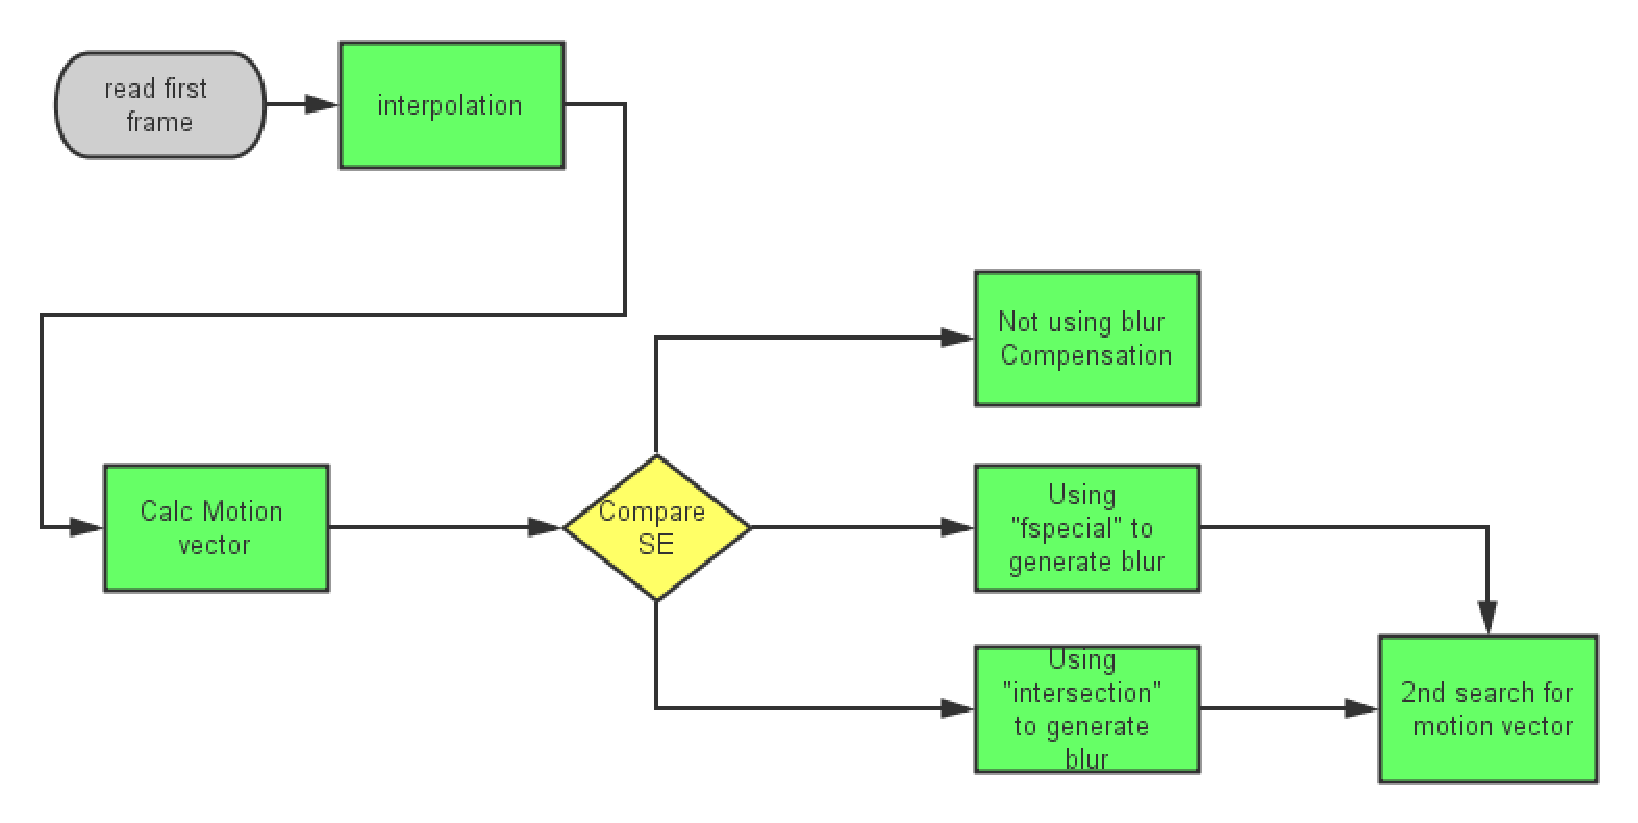
\includegraphics[width=4in]{flowc.pdf} 
   \caption{the flowchart of the proposed algorithm of motion blur compensation}
   \label{flow}
\end{figure}

\section{Experimental results}


We use a viedo clip named 'playground.yuv' which contains a swinging girl which is blurred because of fast motion relative to the camera. and takes 25 consecutive frames from it to test our proposed algorithm. 

Overall, the proposed algorithm reduces 7.5\% SE compared to only using motion compensation. On the other hand, only using fspecial or intersection reduces only 6.6\% SE and 6.4\% SE, respectively.

The result in figure [\ref{compare}] indicates that in some frames the 'fspecial' method is better (e.g. the 38th frame)while in others(e.g. the 32th frame), 'intersection' is better and that is the reason we combine the two methods together.

The PSNR result in figure [\ref{psnr}] is interesting. Both motion compensation and blur compensation give lower PSNR than usual in the prediction of using 39th frame to estimate the 40th frame. It is because the 39th frame suffer from a globel blur perhaps due to the shake of the camera but the 40th frame is normal, and it is hard to use a blurred frame to compensate for a sharp frame in the proposed algorithm. Deblur algorithm might be included to handle this situation in further research.



\begin{figure}
   \centering
   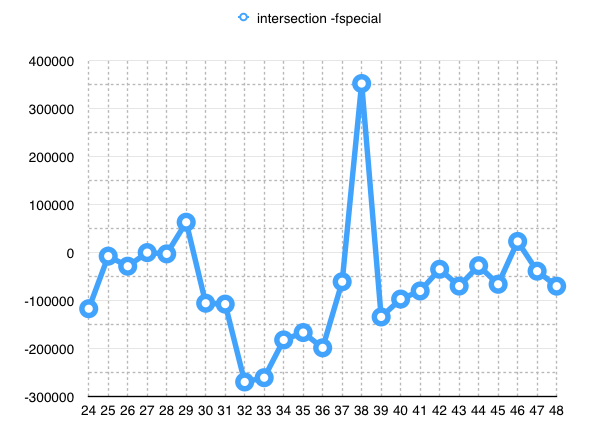
\includegraphics[width=4in]{compare-fspe-interse.png} 
   \caption{A comparison between fspecial PSF and intersection PSF, the value on Y axis represents the SE using intersection minus the SE using fspecial. they both have advantages}
   \label{compare}
\end{figure}
\section{Next steps}

One possible direction is to locate the blurred region first and then applying blurring compensation because it will save the computational cost by give up trying to apply blur compensation to the sharp region of a frame. \cite{Chakrabarti:cb} proposed an algorithm to get the segmentation of the non-uniform blurrd region of a single image by combining the blur cue and colour information, but it is limited to only horizongtal and vertical motion blur. Following this work, \cite{CouzinieDevy:2013bf} proposed an deblurr algorithm based on blur area segmentation.


Another possible direction is using phase correlation for blur compensation. Firouzi proposed an phase correction based algorithm to detect the blur region and blur parameter for video coding in\cite{Firouzi:2014tf}. But his experiment dataset contains only synthesized photos and it awaits validation on real world videos.

\begin{figure}
 \centering
   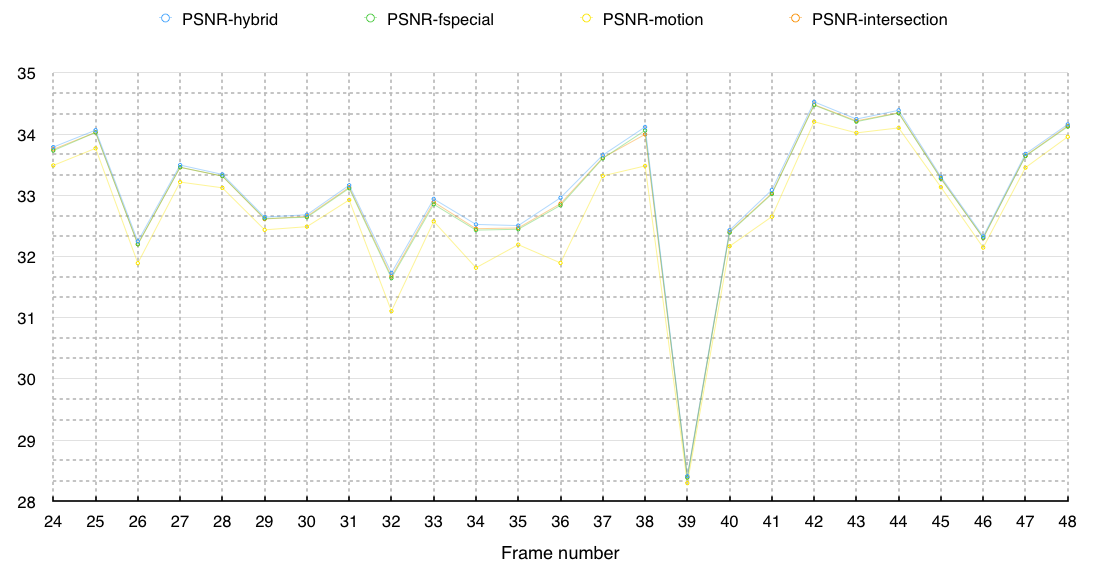
\includegraphics[width=6in]{psnr.png} 
   \caption{The PSNR of using blur compensation and only motion compensation}
   \label{psnr}
\end{figure}

\begin{thebibliography}{99}
\bibitem{intersection}Oliveira, J. P., Figueiredo, M. A. T., \& Bioucas-Dias, J. M. (n.d.). Parametric Blur Estimation for Blind Restoration of Natural Images: Linear Motion and Out-of-Focus. IEEE Transactions on Image Processing, 23(1), 466–477. doi:10.1109/TIP.2013.2286328
\bibitem{Chakrabarti:cb}Chakrabarti, A., Zickler, T., \& Freeman, W. T. (n.d.). Analyzing spatially-varying blur (pp. 2512–2519). Presented at the 2010 IEEE Conference on Computer Vision and Pattern Recognition (CVPR), IEEE. doi:10.1109/CVPR.2010.5539954
\bibitem{CouzinieDevy:2013bf}Couzinié-Devy, F., Sun, J., \& Alahari, K. (2013). Learning to estimate and remove non-uniform image blur. Computer Vision and …. doi:10.1109/CVPR.2013.143
\bibitem{Firouzi:2014tf}Firouzi, S. (2012). Blur Compensation in Predictive Video Coding, 1–131.
\bibitem{Tai:2013db}Tai, Y.-W., Chen, X., Kim, S., Kim, S. J., Li, F., Yang, J., et al. (2013). Nonlinear Camera Response Functions and Image Deblurring: Theoretical Analysis and Practice. IEEE Transactions on Pattern Analysis and Machine Intelligence, 35(10), 2498–2512. doi:10.1109/TPAMI.2013.40
\bibitem{Anonymous:9rR77Z_8}Laude, T., Meuel, H., Liu, Y., \& Ostermann, J. (n.d.). Motion Blur Compensation in Scalable HEVC Hybrid Video Coding. Tnt.Uni-Hannover.De
. 
\end{thebibliography}
\end{document}